This section provides a conceptual framework for understanding changes in birth spacing.
I first introduce three potential explanations that link fertility and birth 
spacing decisions: economic conditions, desired child outcomes, and son preference 
\citep{Casterline2016,Portner2018}.
Next, I discuss why female education and area of residence are the principal factors 
in the empirical analyses and how they tie into the three explanations.

% Economic conditions
The improvements in economic condition, especially the doubling of real wages,
are likely to affect fertility although the direction is ambiguous; empirically, 
higher female wages lowers fertility, whereas higher male wages increases fertility 
\citep{Hotz1997,schultz97}.
Economic theory predicts that the effect of higher wages on fertility is determined by 
the relative strengths of the substitution and income effects.
The substitute effect captures that as wages increase time becomes more expensive, and
people therefore work more and spend less time on non-wage earning activities, such as 
children or leisure.
The income effect captures that higher wages increase the available income, which
leads people to spend more time on time-intensive activities and less time working.
Since women spend substantially more time on childrearing than men, the substitution effect 
dominates for women but the income effect for men.

Higher female wages will also tend to shorten birth spacing if having children requires 
the mother to curtail her economic activities.
Shortening birth spacing allows parents to take advantage of economies of scale in 
childrearing---for example, looking after two children requires less than double the time 
needed for one child \citep{Vijverberg1982,Hotz1997}.


% Child outcomes
Parents care both about how many children they have and their outcomes, and with 
increasing returns to education and lower offspring mortality, parents are likely to 
reduce fertility and invest more in each child \citep{Rosenzweig1982a,Wolpin1997}.
The higher return to education means a stronger incentive to invest in their children's
education, which increases the cost of children and lowers fertility. 
With lower expected mortality fewer births are required to reach a desired number 
of surviving children, which furthermore allows parents to invest more in each child.

An increased desired for better child outcomes will also tend to lengthen birth spacing,
provided it has positive effects on child outcomes.
The clearest example of a positive effect of longer spacing that very short 
spacing---approximately 24 months or less---leads to worse child health and mortality 
outcomes \citep{Whitworth2002,Conde-Agudelo2012}.
Whether longer spacing also improves human capital outcomes is more speculative with
mixed evidence for developed countries and no evidence for developing countries
\citep{Zajonc1976,Powell1993,Pettersson-Lidbom2009,Buckles2012,Barclay2017}.

% Son preference 
Empirically, stronger son preference only marginally increases average fertility, but
differential stopping behavior still affects the sex composition and fertility across 
families and leads to shorter spacing and worse health outcomes for daughters  
when there are no sons in the household
\citep{repetto72,clark00,Whitworth2002,Basu2010,Jayachandran2011,Barcellos2014}.
 
Stronger son preference increases the use of sex selection and each sex-selective
abortion increases the expected birth spacing by 6--12 months.
After an abortion the uterus needs at least two menstrual cycles---approximately 
two months---to recover, or the subsequent risk of spontaneous abortion increases 
substantially \citep{zhou00b}.
Once conception can be attempted, the waiting time to conception is likely between
one and six months. 
Finally, sex-determination tests are reliable only from three months of gestation. 
Hence, it takes at least six months before the couple is at the same point in the next 
pregnancy as they were in the prior pregnancy when they decided to abort.

The use of sex selection, and therefore the length of birth intervals, increases with
lower desired fertility and with parity, provided the desired number of sons has 
not been reached \citep{Portner2015b,Jayachandran2017}.  

% Factors/predictions
Although the explanations above are based on economic conditions, desired child outcomes,
son preference, and sex selection, none of these are available in the data, so I instead 
use female education and area of residence as the two principal explanatory variables in 
the empirical analyses.
Not only are these the closest available proxies, prior research shows that both higher 
female education and urbanization are associated with lower fertility and increased 
sex selection use, and, therefore, likely also changes birth spacing
\citep{das_gupta97,dreze01,bhat03,retherford03b,Guilmoto2009a,Portner2015b,Jayachandran2017}.
Furthermore, both variables are of interest given the tremendous changes in India; 
Figure \ref{fig:education_over_time} shows the substantial increase in female education
and the urban proportion of the population almost doubled from 18\% in 1960 to 35\% in 
2019 \citep{United-Nations2019}.

\begin{figure}[htpb]
\centering
\subfloat[Rural]{
    \begin{minipage}{0.49\textwidth}
        
\includegraphics[width=\textwidth]{educ_over_time_rural}
    \end{minipage}
} 
\subfloat[Urban]{
    \begin{minipage}{0.49\textwidth}
        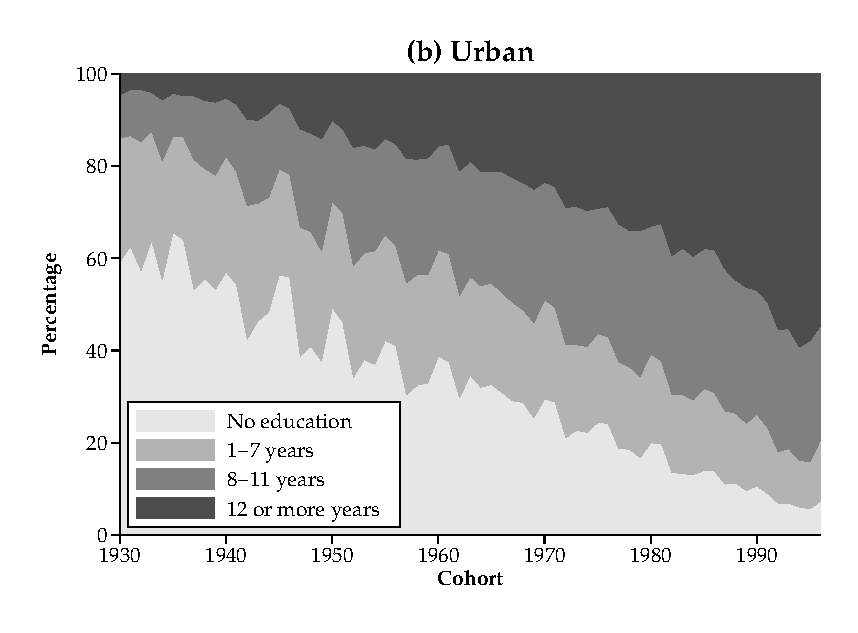
\includegraphics[width=\textwidth]{educ_over_time_urban} 
    \end{minipage}
}
\caption{Distribution of education by cohort for women 20 years or older
using the four rounds of the NFHS}
\label{fig:education_over_time}
\end{figure}


Urban women are likely to have lower fertility and higher use of sex selection than women 
in rural areas.
The lower fertility is the result of higher cost of children and lower child mortality 
risk in urban compared to rural areas.%
\footnote{
However, holding parental education constant, children in Indian slums have worse
health outcomes than in rural areas \citep{Portner2018a}.
}
The higher use of sex selection comes partly from the lower fertility and partly from
higher income and better access to health care facilities in urban areas.

As women receive more education their potential wages increase, which should shorten 
birth spacing and lower fertility, but the low and declining female labor force 
participation in India suggests that families face little incentive to space children 
more closely together for economic reasons.
Even as women's education increased, their labor force participation stagnated or 
decreased and is now one of the lowest outside the Middle East 
\citep{Klasen2015,Fletcher2017,Afridi2018,Bhargava2018,Chatterjee2018}.

The decline in female labor force participation appear to be driven by a combination
of a relatively small expansion in the sectors where women work and the income effect 
from rapidly increasing male wages and education dominating the substitution effect from 
higher female wages \citep{Klasen2015,Bhargava2018}.
The income effect can dominate because not only do men have a higher average level of 
education than women, men are also paid more than women for a given level of education, 
and the returns to education increases with education in India \citep{Agrawal2011}.
Hence, increasing male education will result in an larger increase in income than a 
similar increase in female education.

However, in a situation with increasing returns to male education and declining female labor 
force participation, we might still observe an association between higher female education 
and both lower fertility and increased use of sex selection, provided better-educated women 
are better at producing child human capital as suggested by \citet{Behrman1999}.
In this scenario, better-educated women are desired not for their ability to generate
income but for their ability to produce better-educated sons.
The higher return to male education provides an additional incentive to invest in sons'
education---with a better-educated mother one such investment---and also lowers desired 
fertility, makes sex selection more likely, and possibly increases birth spacing.

% Sanskritization
Finally, although the expansion in female education will likely bring in groups who 
initially have different norms, the process of ``Sanskritization'' implies that as 
lower-castes females gain access to education, they adopt higher-caste norms such as stronger son 
preference and a retraction from the formal labor market \citep{Srinivas1956}.
The declining female labor force participation suggests that this process still 
operates \citep{Abraham2013,Chatterjee2018}.

% Summary / hypotheses
In summary, with substantial increases in husbands' income and a declining female labor 
force participation, I expect longer birth spacing over time, independent of education 
levels.
Furthermore, birth spacing likely increases the most among the better educated 
because their household income increases the most---even with declining female labor 
participation---and because of their use of sex selection.
Finally, "Sanskritization" implies that the changing composition of better-educated
women will not substantially change the use of sex selection.






